\section{Klassediagrammer}\label{Klassediagrammer}
\externaldocument{appendix}
For at få et overblik over program delene der skulle til for at kunne løse problemet, er der løbende blevet opstillet klassediagrammer. De følgende diagrammer er de endelige udgaver, under udformningen af programmet er der blevet ændret, tilføjet og fjernet forskellige klasser som diskuteres i afsnit \textbf{REF}. Klassediagrammerne for brugerfladen er ikke vist her, men kan findes i bilag \ref{AppendixA} og \ref{AppendixB}.

\vspace{5mm}

I diagrammerne betyder skråtekst at klassen er abstrakt, plus er et offentligt medlem, minus er et privat medlem, hashcode er et beskyttet (protected) medlem og understregning betyder at medlemmet er statisk. Hver klasse har tre kasser, den første indeholder klassens navn, den anden kasse består af klassens fields, og den sidste indeholder klassens properties, metoder og events.

\begin{figure}[H]
    \centering
    \makebox[\textwidth][c]{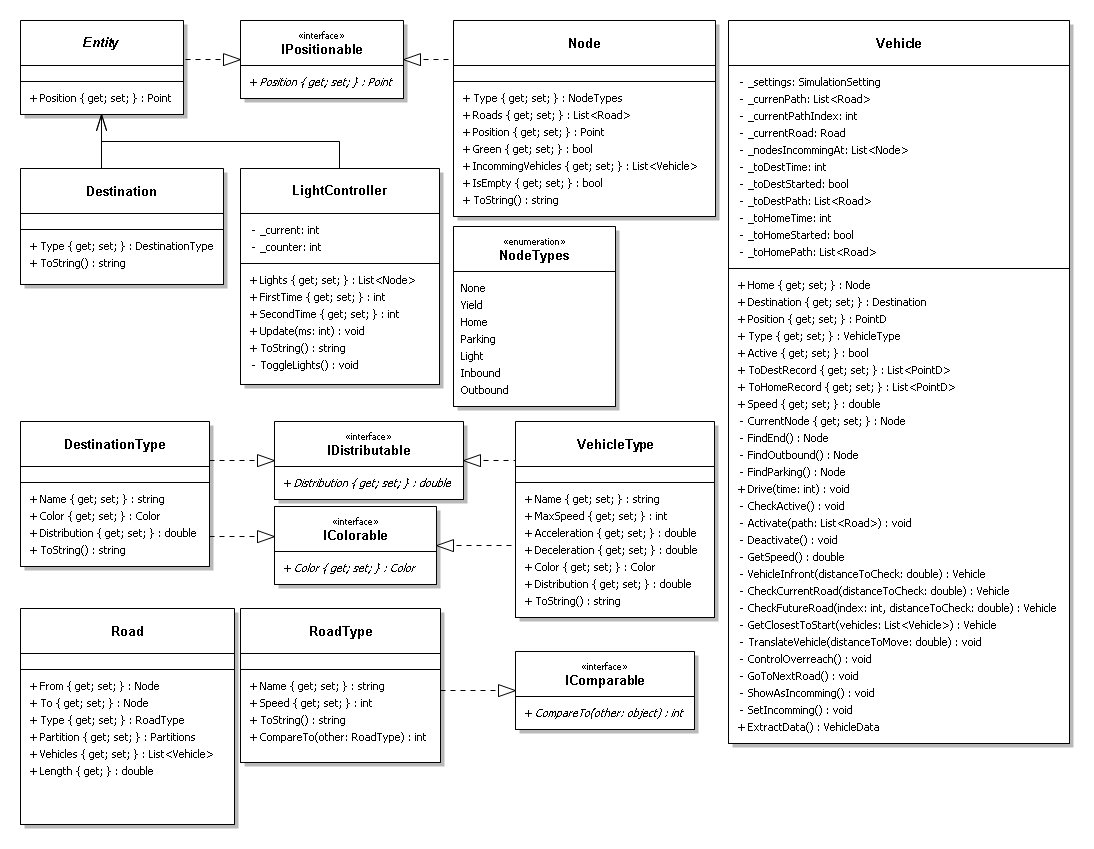
\includegraphics[width=1.4\textwidth,height=\textheight,keepaspectratio]{Pictures/Klassediagram/VejElementer}}
    \caption{Elementer i vejnettet}
    \label{kdVejElementer}
\end{figure}

Diagrammet der ses på figur \ref{kdVejElementer} indeholder alle klasserne der er en del af vejnettet. Elementerne der arver fra den absktrakte klasse \texttt{Entity}, er elementer der kan positioneres, men ikke forbindes med vejnettet. \texttt{Node} klassen er de noder vejne kan forbindes imellem. \texttt{Road} klassen beskriver vejene køretøjerne kan bevæge sig langs. \texttt{Vehicle} klassen beskriver et køretøj, og hvordan hastighed og bevægelsen skal foregå. \texttt{Destination}, \texttt{Road} og \texttt{Vehicle} klasserne har hver især en tilsvarende type-klasse, som brugeren kan lave nye instanser af og dermed bestemme elementernes egenskaber. Elementerne i dette diagram bliver uddybet på i afsnit \ref{ElementerVejnettet}, bortset fra \texttt{Vehicle} der bliver forklaret i afsnit \ref{Vehicle}.

\begin{figure}[H]
    \centering
    \makebox[\textwidth][c]{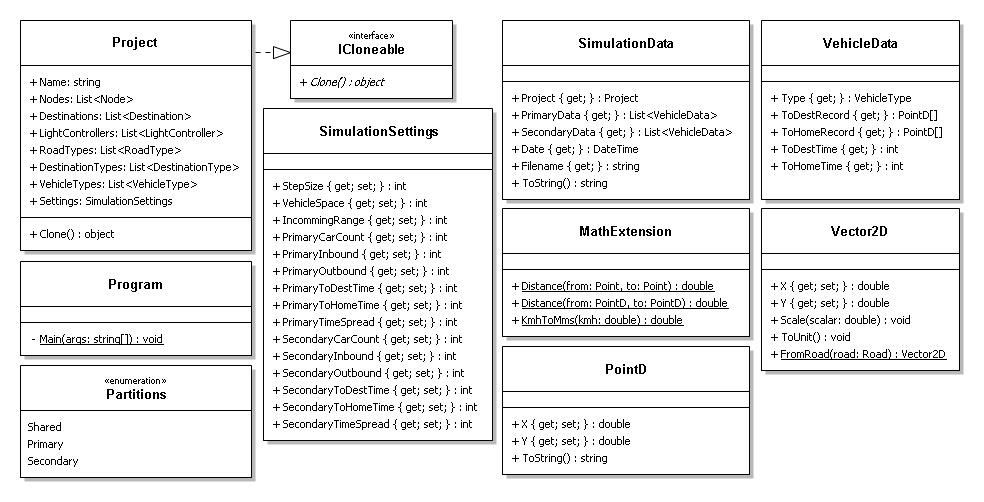
\includegraphics[width=1.4\textwidth,height=\textheight,keepaspectratio]{Pictures/Klassediagram/Diverse}}
    \caption{Diverse klasser}
    \label{kdDiverse}
\end{figure}

På figur \ref{kdDiverse} ses diagrammet for nogle forskellige klasser der ikke ligger under en bred kategori. \texttt{Project} klassen indeholder alt informationen om brugerens indstillinger og brugerens opbyggede vejnet. \texttt{SimulationData} indeholder en klon af projektet fra det tidspunkt det blev simuleret, og en optagelse af den positionelle data fra \texttt{Vehicle} instanserne der befærdede sig på vejnettet. \texttt{Partitions} er en enumerator der bliver brugt forskellige steder gennem programmet til at skelne mellem den primære og den sekundære simulering. \texttt{PointD} er en klasse der beskriver et punkt med doubles, for ikke at miste præcision ved at konvertere mellem floats og doubles. Den statiske klasse \texttt{MathExtension} indeholder nogle formler der ikke findes i standard biblioteket \texttt{Math}. \texttt{Vector2D} beskriver en vektor, og har nogle hjælpe metoder til at arbejde med vektorer. Disse klasser bliver uddybet i afsnit \ref{Diverse}.

\begin{figure}[H]
    \centering
    \makebox[\textwidth][c]{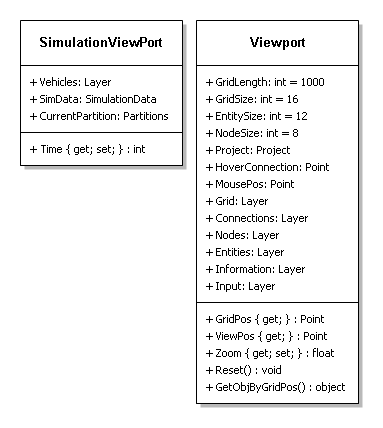
\includegraphics[width=1.4\textwidth,height=\textheight,keepaspectratio]{Pictures/Klassediagram/Viewport}}
    \caption{Viewport og SimulationViewport}
    \label{kdViewport}
\end{figure}

De to klasser på figur \ref{kdViewport} er brugerflade elementerne hvor brugeren kan se vejnettet. Den første klasse \texttt{Viewport}, er den der ses i programmets hoved brugerflade \texttt{GUIMain}, hvor der kan redigeres i vejnettet. Klassen \texttt{SimulationViewport} arver fra Viewport, og bruges til at vise hvordan køretøjerne bevæger sig. Disse klasser forklares i afsnit \ref{HovedBrugerfladen}.

\begin{figure}[H]
    \centering
    \makebox[\textwidth][c]{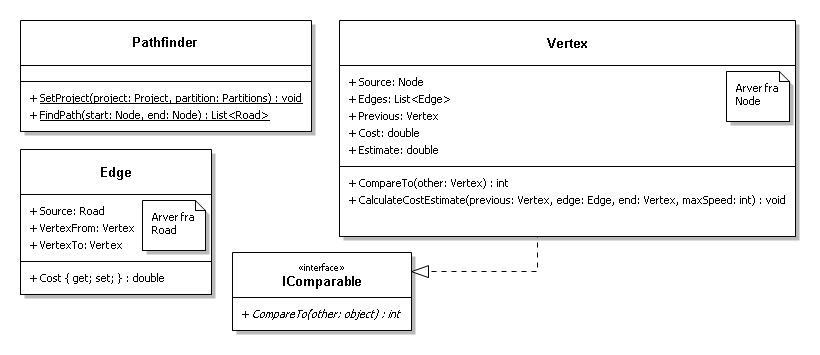
\includegraphics[width=1.4\textwidth,height=\textheight,keepaspectratio]{Pictures/Klassediagram/Pathfinder}}
    \caption{Pathfinder klassen}
    \label{kdPathfinder}
\end{figure}

\texttt{Pathfinder} klassen, som vises sammen med \texttt{Vertex} og \texttt{Edge} klasserne på figur \ref{kdPathfinder}, bruges hver gang en \texttt{Vehicle} bliver konstrueret. Ved \texttt{Vehicle}'s konstruktion, findes den hurtigste vej til destinationen og ruten tilbage igen, som gemmes i selve \texttt{Vehicle} instansen. \texttt{Vertex} og \texttt{Edge} arver fra \texttt{Node} og \texttt{Road}, og indeholder yderligere informationer som \texttt{Pathfinder} bruger til at finde den optimale rute. \texttt{Pathfinder} beskrives i afsnit \ref{Pathfinder}.

\begin{figure}[H]
    \centering
    \makebox[\textwidth][c]{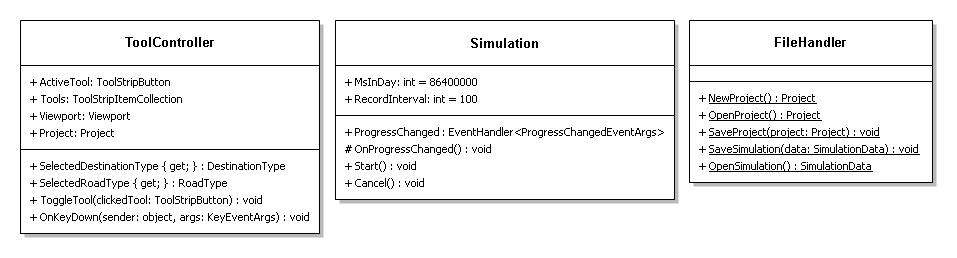
\includegraphics[width=1.4\textwidth,height=\textheight,keepaspectratio]{Pictures/Klassediagram/Funktionalitet}}
    \caption{De funktionelle klasser}
    \label{kdFunktionelle}
\end{figure}

Diagrammet på figur \ref{kdFunktionelle} viser klasserne hvor en stor del af programmets logik bliver håndteret. \texttt{ToolControllerne} modtager input fra \texttt{GUIMain} når der bliver trykket på værktøjsknapperne, og modtager input fra Viewporten når der bliver trykket på gitteret, hvor den så derefter bestemmer hvad der skal ske baseret på det aktive værktøj. \texttt{Simulation} klassen håndterer selve simuleringerne af de primære og sekundære køretøjer, over en periode på 24 timer. \texttt{FileHandler} klassen er statisk og kan gemme og åbne \texttt{Project} klassen og \texttt{SimulationData} klassen. Disse klasser bliver forklaret i afsnit \ref{Funktionelle}.